\documentclass[a4paper,11pt]{article}
\usepackage{amsmath,amsthm,amsfonts,amssymb,amscd,amstext,vmargin,graphics,graphicx,tabularx,multicol} 
\usepackage[francais]{babel}
\usepackage[utf8]{inputenc}  
\usepackage[T1]{fontenc} 
\usepackage{pstricks-add,tikz,tkz-tab,variations}
\usepackage[autolanguage,np]{numprint} 

\setmarginsrb{1.5cm}{0.5cm}{1cm}{0.5cm}{0cm}{0cm}{0cm}{0cm} %Gauche, haut, droite, haut
\newcounter{numexo}
\newcommand{\exo}[1]{\stepcounter{numexo}\noindent{\bf Exercice~\thenumexo} : \marginpar{\hfill /#1}}
\reversemarginpar


\newcounter{enumtabi}
\newcounter{enumtaba}
\newcommand{\q}{\stepcounter{enumtabi} \theenumtabi.  }
\newcommand{\qa}{\stepcounter{enumtaba} (\alph{enumtaba}) }
\newcommand{\initq}{\setcounter{enumtabi}{0}}
\newcommand{\initqa}{\setcounter{enumtaba}{0}}

\newcommand{\be}{\begin{enumerate}}
\newcommand{\ee}{\end{enumerate}}
\newcommand{\bi}{\begin{itemize}}
\newcommand{\ei}{\end{itemize}}
\newcommand{\bp}{\begin{pspicture*}}
\newcommand{\ep}{\end{pspicture*}}
\newcommand{\bt}{\begin{tabular}}
\newcommand{\et}{\end{tabular}}
\renewcommand{\tabularxcolumn}[1]{>{\centering}m{#1}} %(colonne m{} centrée, au lieu de p par défault) 
\newcommand{\tnl}{\tabularnewline}

\newcommand{\bmul}[1]{\begin{multicols}{#1}}
\newcommand{\emul}{\end{multicols}}

\newcommand{\trait}{\noindent \rule{\linewidth}{0.2mm}}
\newcommand{\hs}[1]{\hspace{#1}}
\newcommand{\vs}[1]{\vspace{#1}}

\newcommand{\N}{\mathbb{N}}
\newcommand{\Z}{\mathbb{Z}}
\newcommand{\R}{\mathbb{R}}
\newcommand{\C}{\mathbb{C}}
\newcommand{\Dcal}{\mathcal{D}}
\newcommand{\Ccal}{\mathcal{C}}
\newcommand{\mc}{\mathcal}

\newcommand{\vect}[1]{\overrightarrow{#1}}
\newcommand{\ds}{\displaystyle}
\newcommand{\eq}{\quad \Leftrightarrow \quad}
\newcommand{\vecti}{\vec{\imath}}
\newcommand{\vectj}{\vec{\jmath}}
\newcommand{\Oij}{(O;\vec{\imath}, \vec{\jmath})}
\newcommand{\OIJ}{(O;I,J)}


\newcommand{\reponse}[1][1]{%
\multido{}{#1}{\makebox[\linewidth]{\rule[0pt]{0pt}{20pt}\dotfill}
}}

\newcommand{\titre}[5] 
% #1: titre #2: haut gauche #3: bas gauche #4: haut droite #5: bas droite
{
\noindent #2 \hfill #4 \\
#3 \hfill #5

\vspace{-1.6cm}

\begin{center}\rule{6cm}{0.5mm}\end{center}
\vspace{0.2cm}
\begin{center}{\large{\textbf{#1}}}\end{center}
\begin{center}\rule{6cm}{0.5mm}\end{center}
}



\begin{document}
\pagestyle{empty}
\titre{Interrogation: Longueur, milieu et distance}{Nom :}{Prénom :}{Classe}{Date}


\exo{1} Cours \\

\noindent Donner la définition du milieu d'un segment.\\
\reponse[3]\\




\exo{3} Écrire les codages manquants sur chacune des figures

\bmul{2}

\q On sait que : \\

 \noindent - O est le milieu de [AC],\\
 -  OB = OA \\
 - $(AB) \perp (BC)$\\


\columnbreak

\includegraphics[scale=1]{codage.eps} 

\emul

\bmul{2}

\q On sait que : \\
\noindent - LP = PE = EL\\
 - ME = MU \\
 - $(LE) \perp (LM)$ \\
 - $(LM)  \perp (MU) $\\


\columnbreak

\includegraphics[scale=0.5]{codage1.eps} 

\emul


\medskip

\exo{2}

\bmul{2}

Placer  les  points  A,  B,  C,  D  et E sur la figure suivante sachant que : \\

 \noindent - E est le milieu du segment [BC], \\
- $(AC) \perp (BC)$ \\
- AD = BD \\

\columnbreak

\includegraphics[scale=0.6]{codage2.eps} 

\emul


\exo{4}\\
Tracer  un segment [FG] tel que : FG = 15 cm.\\
Placer C, le point du segment [FG] tel que : FC = 6,4 cm.\\
Placer M, le milieu du segment [FC].\\
Placer K, le point du segment [FG] tel que : C est le milieu de [FK]. \\


\initq \q Faire une figure.\\

\newpage

\vspace*{0.5cm}


\q Calculer CG. (Justifier votre réponse.)\\
\reponse[5]\\

\vspace*{0.3cm}

\q Calculer FM. (Justifier votre réponse.)\\
\reponse[5]\\

\end{document}
